The Eternal Webpages package is a Proof Of Concept package no longer undergoing 
active development. Its main purpose is to download and bundle resources referenced by a webpage
in such a way that they can be fetched offline.
To accomplish this, the webbrowser has 2 modes for viewing websites: one by browsing
the internet and one by downloading P2P cached copies of websites (called internet viewmode and
swarm viewmode respectively). This is shown in \autoref{fig:activitybrowsing}.
The package is referenced from the main Tribler projects web browser for every resource
it ecounters while loading a webpage. This is shown in \autoref{fig:activityseeding}.
The full class diagram of the package is included in \autoref{fig:classdiagrameternalweb}.

\begin{figure}[h]
  \centering
      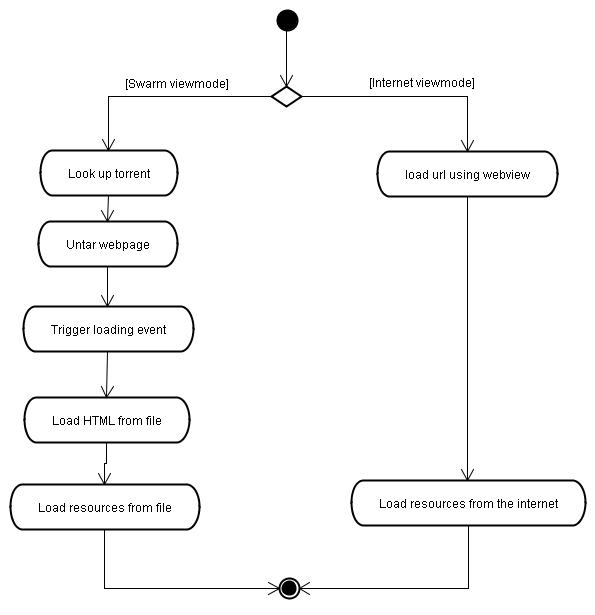
\includegraphics[width=0.8\textwidth]{SiteRipper-Browsing-activitydiagram.jpg}
  \caption{Activity diagram of viewmode based webbrowsing}
  \label{fig:activitybrowsing}
\end{figure}

\begin{figure}[h]
  \centering
      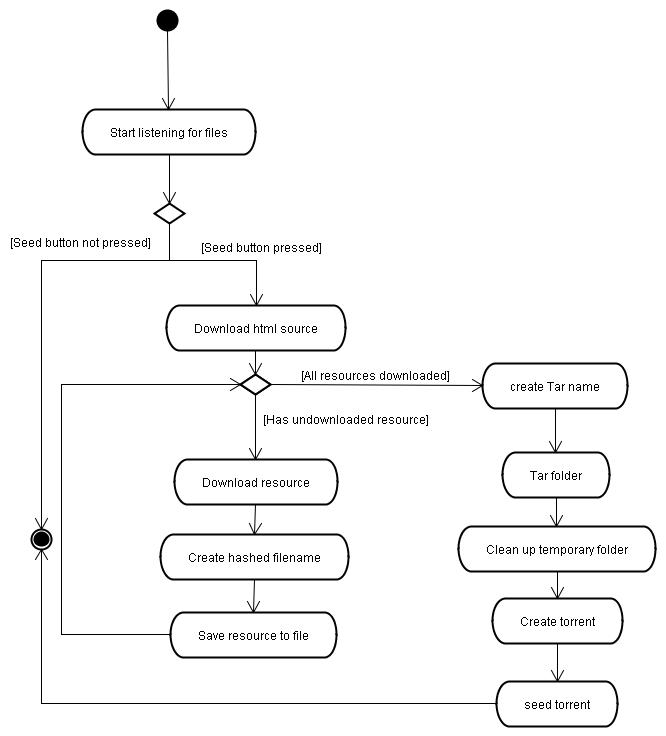
\includegraphics[width=0.8\textwidth]{SiteRipper-Seeding-activitydiagram.jpg}
  \caption{Activity diagram of seeding mode webbrowsing}
  \label{fig:activityseeding}
\end{figure}

\begin{figure}[h]
  \centering
\tikzimgEternalWebpages
  \caption{Class diagram for Eternal Webpages}
  \label{fig:classdiagrameternalweb}
\end{figure}
